\chapter{Setting the Stage}  
\label{chap:prologue} 

Let's first get an overview of the topic and the nature of this book.
Keep in mind, this is just an overview; many questions should come to
your mind, hopefully whetting your appetite for the succeeding chapters!

In this chapter, we will mainly describe \textit{collaborative
filtering}, one of several common approaches to recommender systems
(RTSs). 

\section{What Are Recommender Systems?}

What is an RS?  We're all familiar with the obvious ones---Amazon
suggesting books for us to buy, Twitter suggesting whom we may wish to
follow, even OK Cupid suggesting potential dates. 

But many applications are less obvious.  The University of Minnesota,
for instance, has developed an RS to aid its students in selection of
courses.  The tool not only predicts whether a student would like a
certain course, but also even predicts the grade she would get!

In discussing RS systems, we use the terms \textit{users} and
\textit{items}, with the numerical outcome being
termed the \textit{rating}.  In the famous MovieLens dataset, which
we'll use a lot, users provide their ratings of films.

Systems that combine user and item data as above are said to perform
\textit{collaborative filtering}.  The first part of this book will
focus on this type of RS.  \textit{Content-based} RS systems work by
learning a user's tastes, say by text analysis.

Ratings can be on an ordinal scale, e.g.\ 1-5 in the movie case.  Or 
they can be binary, such as a user clicking a Like symbol in Twitter, 1 for a
click, 0 for no click.

But ratings in RSs are much more than just the question, ``How much do
you like it?''  The Minnesota grade prediction example above is an
instance of this.

In another example, we may wish to try to predict bad reactions to
prescription drugs among patients in a medical organization.  Here the
user is a patient, the item is a drug, and the rating may be 1 for
reaction, 0 if not.  

More generally, any setting suitable for what in statistics is called
a \textit{crossed heirachical model} fits into RS.  The word
\textit{crossed} here means that each user is paired with multiple
items, and vice versa.  The hierarchy refers to the fact that we can
group users within items or vice versa.  There would be two levels of
hierarchy here, but there could be more.  

Say we are looking at elementary school students rating story books.  We
could add more levels to the analysis, e.g. kids within schools within
school districts.  It could be, for instance, that kids in different
schools like different books, and we should take that into account in
our analysis.  The results may help a school select textbooks that are
especially motivational for their students.

Note that in RS data, most users have not rated most items.  If we form
a matrix of ratings, with rows representing users and columns indicating
items, most of the elements of the matrix will be unknown.  We are
trying to predict the missing values.  Note carefully that these are not
the same as 0s.


\section{The ``Hello World'' of RS:  MovieLens}

This dataset is the standard introduction to RSs, and indeed is a
standard example in RS research papers.  It's available from the
GroupLens project at the University of Minnesota, \url{grouplens.org}.
In this book, we will mainly use the 100K version, which contains
100,000 rates in the format

\begin{lstlisting}
userID  movieID  rating1to5  timestamp
\end{lstlisting}

Let's take a look:

\begin{lstlisting}
> download.file('http://files.grouplens.org/datasets/movielens/ml-100k.zip', 
>    'ml-100k.zip') 
> unzip('ml-100k.zip') 
> ml100 <- read.csv('ml-100k/u.data',header=FALSE,sep='\t')
> head(ml100)
   V1  V2 V3        V4
1 196 242  3 881250949
2 186 302  3 891717742
3  22 377  1 878887116
4 244  51  2 880606923
5 166 346  1 886397596
6 298 474  4 884182806
\end{lstlisting}

(Note that the data comes in TAB-separated fields.)

We see for instance user 22 rated movie 377 as 1.  Let's explore some more:

\begin{lstlisting}
> length(unique(ml100$V1))
[1] 943
> length(unique(ml100$V2))
[1] 1682
> table(ml100$V3)

    1     2     3     4     5 
 6110 11370 27145 34174 21201 
\end{lstlisting}

So there were 943 users and 1682 films.  Users seemed to be pretty
liberal in their ratings, with the most popular rating being a 4.

We can break that down by user:

\begin{lstlisting}
> tmp <- tapply(ml100$V3,ml100$V1,mean)
> tmp[22]
      22 
3.351562 
\end{lstlisting}

Here we groped ratings according to age, computing the mean rating for
each age value.

So for instance user 22 gave an average rating of about 3.35 to the ones
he/she rated.  And how many films was that?

\begin{lstlisting}
> tmp <- tapply(ml100$V3,ml100$V1,length)
> tmp[22]
 22 
128 
\end{lstlisting}

Did user 22 rate movie 88?

\begin{lstlisting}
> ml100[ml100$V1 == 22 & ml100$V2 == 88,]
[1] V1 V2 V3 V4
<0 rows> (or 0-length row.names)
\end{lstlisting}

No.  And that is the essence of RS:  How can we predict what rating user
22 would give to that movie?

We can represent our data as a matrix, e.g.

\begin{equation}
\label{ratmat}
\left (
\begin{array}{rrrr}
1 & 5 & 1 & -2 \\
8 & 3 & 2 & 8 \\
9 & 8 & 3 & 6 
\end{array}
\right )
\end{equation}


\section{How Is It Done?}

Putting aside possible privacy issues that arise in some of the above RS
applications,\footnote{I used to be mildy
troubled by Amazon's suggestions, but with the general demise of
browsable bricks-and-mortar bookstores, I now tend to view it as ``a
feature rather than a bug.''} we ask here, How do they do this?  In this
prologue, we'll discuss a few of the major methods for collaborative
filtering (CF)..

\subsection{Nearest-Neighbor Methods}

This is probably the oldest class of RS methodology, still popular
today.  It can be explained very simply.

Say there is a movie spoofing superheroes called \textit{Batman Goes
Batty} (BGB).  Maria hasn't seen it, and wonders whether she would like
it.  To form a predicted rating for her, we could search in our dataset
for the $k$ users most similar to Maria in movie ratings and who have
rated BGB.  We would then average their ratings in order to derive a
predicted rating of BGB for Maria.  We'll treat the issues of choosing
the value of $k$ and defining ``similar'' later, but this is the
overview.

In general, methods like this are called k-NN methods,
for ``k-nearest neighbor.''  (We'll shorten it to kNN.)
Actually, kNN was one of the earliest methods in machine learning in
general.

\subsection{Latent Factor Approach:  Matrix Factorization}
\label{mf}

This one is less intuitive, but is probably the most popular CF methods.

Let $A$ denote the matrix of ratings described earlier, with $A_{ij}$
denoting the rating user $i$ gives to item $j$.  Keep in mind, as noted,
that most of the entries in $A$ are unknown; following R convention,
we'll refer to them as NA, the R-language notation for missing values.  
So for our movie example above, \lstinline{bf{A[22,377] = 1} and
\lstinline{A[22,88] = NA}.

Matrix factorization (MF) methods then estimate all of $A$ as follows.
Let $r$ and $s$ denote the numbers of rows and colums of $A$,
respectively.  In our data above, for example, $r = 943$ and $s = 1682$.
The idea is to find a \textit{low-rank approximation} to $A$:  Using our
known ratings, we find matrices $W$ and $H$, of dimensions $r \times m$
and $m \times s$, each of rank $m$, such that 

\begin{equation}
A \approx WH
\end{equation}

Typically $m << \min(r,s)$.  Software libraries typically take 10 as the
default.

We will review the concept of matrix rank later, but for now the key is
that $W$ and $H$ are \underline{known} matrices, no NA values.  Thus we
can form the product $WH$, thus obtaining estimates for all the missing
elements of $A$.

For our example above, our predicted value for user 22's rating of
moveie 88 would be

\begin{equation}
(WH)_{22,88}
\end{equation}

\subsection{Latent Factor Approach: Statistical Models}

As noted, collaborative-filtering RS applications form a special case of
crossed random-effects models, a statistical methodology.  In that way,
a useful model for $Y_{ij}$, the rating user $i$ gives item $j$, is

\begin{equation}
Y_{ij} = \mu + \alpha_i + \beta_j + \epsilon_{ij}
\end{equation}

a sum of an overall mean, an effect for user $i$, an effect for item
$j$, and an ``all other effects'' term (often called the ``error
term'').

In the MovieLens setting, $\mu$ would be the mean rating given to all
movies (in the ``population'' of all movies, past, present and future),
$\alpha_i$ would be a measure of the tendency of user $i$ to give
ratings more liberal or harsher than the average user, and $\beta_j$
would a measure of the popularity of movie $j$, relative to the average
movie.

What assumptions are made here?  First, $\mu$ is a fixed but unknown
constant to be estimated.  As to $\alpha_i$ and $\beta_j$, one could on
the one hand treat them as fixed constants to be estimated.  On the
other hand, there are some advantages to treating them as random
variables, we will be seen in Chapter \ref{chap:mixed}.

It is customary to use the ``hat'' notation $\widehat{}$ to mean
``estimate of.''  After finding estimates of the above model quantities
from our data, our predicted value for user 22 and movie 88 would then
be

\begin{equation}
\widehat{A}[22,88] = \widehat{\mu} + \widehat{\alpha}_{22} + 
\widehat{\beta}_{88}
\end{equation}

\subsection{Variety Is Good}

Why so many methods?  There is no perfect solution, and each has
advantagages and disadvantages. 
Some methods may do better than
others on specific datasets.  Some methods take more computation time
than others.  Some methods are hard to explain to nontechnical people.

It's good, therefore, to have a variety of methods in our toolbox.

\section{Tuning Parameters}

The reader is likely familiar with histograms.  Recall that the analyst
must choose a bin width, or similarly, the number of bins.  Here there
is a tradeoff:

\begin{itemize}

\item If the width is too small, some bins will have no data points, or
very few.  We intuitively feel that small samples are not likely to be
accurate, and we will get a histograms that has a very choppy appearance.
For instance, 

\begin{lstlisting}
> tmp <- tapply(ml100$V3,ml100$V1,mean)
> hist(tmp,breaks=15)
> hist(tmp,breaks=50)
\end{lstlisting}

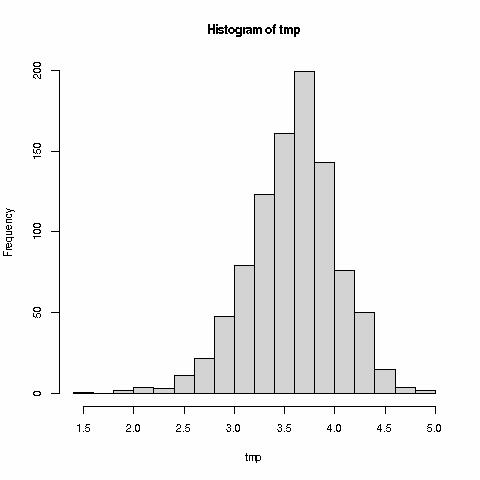
\includegraphics[width=3.5in]{Images/HistBrks15.png} 
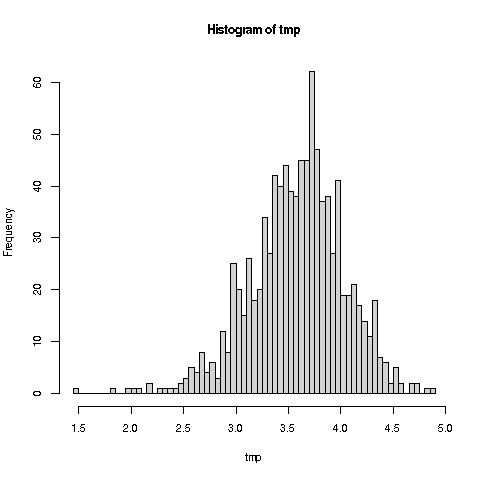
\includegraphics[width=3.5in]{Images/HistBrks50.png} 

\item But it's also bad to have too large a width.  In the extreme, we
have bins so wide that we have just one or two of them; a 2-bin plot
would be of very limited usefulness, and a 1-bin plot would be
totally uninformative:

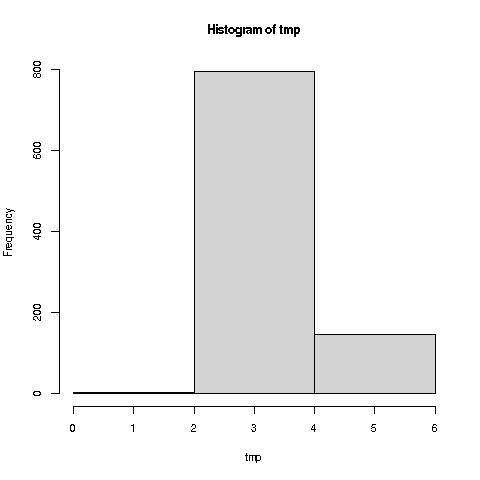
\includegraphics[width=3.5in]{Images/HistBrks2.png} 
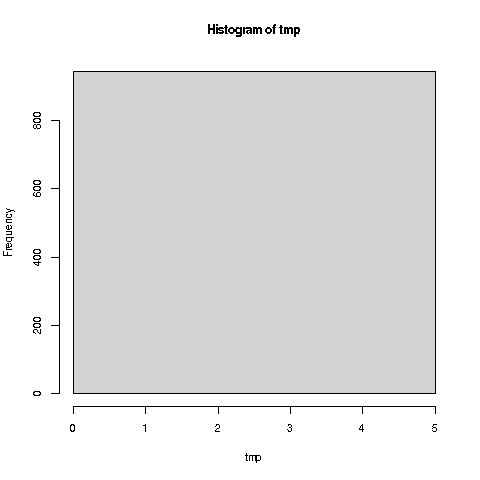
\includegraphics[width=3.5in]{Images/HistBrks1.png} 

\end{itemize} 

The bin width is called a \textit{tuning parameter} or a
\textit{hyperparameter}.  In kNN, the number of neighbors $k$ is the
tuning parameter, and in MF applications, it's the matrix rank $m$.
Most machine learning algorithms, including most in recommender systems,
have tuning parameters, even 10 or more.  Choosing the values of those
parameters is not easy, but there are methods for it, as we will see.

\textbf{Important note:} Think of plotting a histogram for datasets A
and B, similar but A having only 25 data points and B having 500.  With
dataset B, can afford to make the bin width smaller than with dataset A,
as the problem of having empty or nearly-empty bins is much less of an
issue.  Of course, at a certain point, the number bins will be too large
even with B, but the point is that optimal values of tuning parameters
depend on the size of our dataset (as well as various other factors).

By the way, the latent-variable statistical model we introduced earlier
has no tuning parameters.  That may seem tempting, and the model
certainly has various advantages.  But a tuning parameter gives an
opportunity to \textit{tune}, to seek the most accurate model possible.

\section{Covariates/Side Information}

In predicting the rating for a given (user,item) pair, we may for
example have demographic information on the user, such as age and
gender.  Incorporating such information --- called \textit{covariates}
in statistics and \textit{side information} in machine learning --- may
enhance our predictive ability, especially if this user has not rated
many items yet.

However, making good use of side information may not be so easy, for a
couple of reasons:

\begin{itemize}

\item The exact nature of a relationship may not be very clear.  In the
movie example, for instance, we might think that age is an important
factor.  Let's take a quick look, using an extended version of
\lstinline{ml100} obtained from others in the downloaded data (details
not show for now):

\begin{lstlisting}
> w <- tapply(ml100kpluscovs$rating,ml100kpluscovs$age,mean)
> plot(w)
\end{lstlisting}

\begin{figure}[tp]
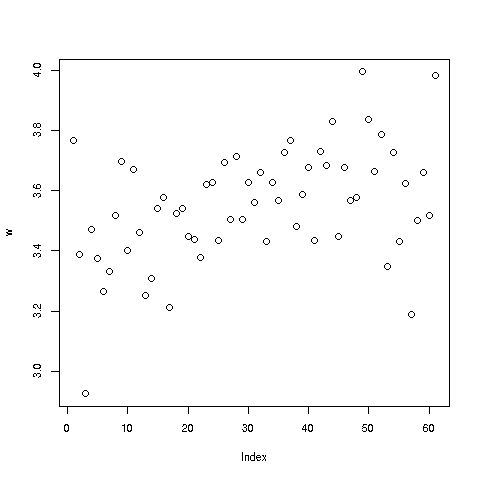
\includegraphics[width=3.5in]{Images/MeanRatVsAge.png} 
\caption{Rating vs.\ Age}
\label{mightlintrend}
\end{figure}

Yes, there does seem to be an upward age trend.  But is it turning
downward at the older ages?

\item And that relationship may not even be useful.  After all, if some
user has rated a large number of films, this data already tells us a lot
about this user's taste in movies.  For that reason, information about
this user's age may be redundant.

\end{itemize} 

No easy answers in predictive data modeling!

\section{Overfitting, Holdout Sets and Cross-Validation}

A major issue---some would say THE major issue---in predictive
data modeling is \textit{overfitting}.  Professor Yaser
Abu-Mostafa of Caltech, a prominent ML figure, once summed it up: ``The
ability to avoid overfitting is what separates professionals from
amateurs in ML.''\footnote{https://www.youtube.com/watch?v=EQWr3GGCdzw}
And my Google query on ``overfitting'' yielded 6,560,000 results!

The concept refers to fitting an overly-complex model to our data.
Consider Figure \ref{mightlintrend}, for example.  We might fit a
straight line, and do fairly well.  But noting a possible dip in trend
near the right side, we could fit a parabola, i.e.\  a quadratic model,
And why stop there?  We could try polynomials of degree 3, 4 and so on.

In fact, a polynomial of degree 60 would give an exact fit, with all 61
points lying on the curve.\footnote{A degree-60 model has 62 parameters,
including the constant term.} But clearly, it would be absurd to do
this, as bad as our example above of a histogram with just one or two
bins.

And indeed, the analogy to the histogram case is strong.  Our polynomial
degree $d$ here is a tuning parameter.  Too large a value, or one that
is too small, won't work well.

In prediction applications, the definition of ``won't work well'' is
that our predictions of new cases in the future won't be very accurate.
Referring to our dataset as the \textit{training data} (``train'' as in
``learn'' in ``machine learning''), we say that we overfit our model to
the training data.  

So, we need some new data.  If we had some, we would take each of our
candidate models---one model for each degree we try---and see which
one predicts best on the new data.

Well, we often don't have new data yet, so we create some.  Before
fitting our models, we set aside some of our data.  We call this the
\textit{holdout set}, and take the rest of our data as the training set.
We fit our various candidate models on this training set, then use each
of the fitted models to predict the holdout set.  Whichever candidate
model does best will then be our choice for prediction on further cases
in the future.

But...by coincidence, the particular holdout set that we form could be
biaed in favor of one model or another.  So, we try many holdout sets,
randomly chosen.  This of course also means many training sets.  For
each training/holdout set pair, we fit all of our candidate models.  In
the end, we take as our final choice whichever model does best over all
the holdout sets.

\section{``P-Hacking,'' Roundoff Error Etc.}

To give a somewhat frivolous example that still will make the point,
say we are investigating whether there is any genetic component to a
person's sense of humor.  Is there a Humor gene?  There are many, many
genes to consider.  Say we have data on 100 people, with some kind of
measurement on ``humorosity'' of each one, plus genetic data on each
person.

There are tons of genes to check.  For each gene, we could compare the
humorosity of people with the gene and people not having the gene (say,
having a particular mutation).  Since we have a random sample of people,
our data is random.  The key point is that \textit{just be accident, by
coincidence, there may be one gene that seems to separate the humorous
people from the dull ones}, when in fact there is no Humor gene.
Conducting a statistical study involving very large numbers of variables
without concern regarding the above possible scenario is called
\textit{p-hacking}.\footnote{The etymology need not concern us here, but
for the curious:  Statistical hypothesis testing---itself methdology
that is the subject of much criticism, rightly so---leads to something
called a p-value.  In the genetics example, the analyst would look for
small p-values, and declare an important discovery if they find one for
some gene.}

In the ML context, we (should) worry about p-hacking if we have a large
number of potential predictor variables (textit{features}, in ML
parlance).  In order to avoid overfitting, we may wish to pare down our
feature set, e.g.\ retain age as a predictor but discard gender.  Denote
the number of predictors by $p$.  (Standard notation, not related to the
first letter in ``p-values.'')  We have $2^p$ possible subsets to
retain.  Even with modest value of $p$, say 10, that's a lot of subsets!
By accident, one might seem to predict better on the holdout sets.

There is no magic solution to this problem (or lots of other problems in
predictive modeling).  Granted,
there are techniques called \textit{multiple inference} or
\textit{multiple comparison} methods, to avoid p-hacking in performing
statistical inference.  See for example \textit{Multiple Comparisons:
Theory and Methods}, Jason Hsu, 1996, CRC.  But these are difficult to
apply, and generally have retrictive assumptions.  

Similarly, many ML methods involve computations involving huge matrices,
with, say, millions of rows and thousands of columns.  Say we wish to
find the inverse (or similar entity) of a huge matrix.  Not only will
the computation take a long time, but also the cumulative roundoff error
could be quite substantial.  Can we trust the result?

Again, there are no magic solutions.  However, with experience one will
develop ways to assess possible problems like these, and deal with them.
Note that ``dealing with them'' may simply mean treating our results as
useful but not infallible---a good viewpoint in any case.

